\subsection{Implementationen}
In diesem Abschnitt sind einzeln konkrete Umsetzungen von Anforderungen aufgeführt und über Commit-IDs oder Branch-Namen weiter referenziert.

\subsubsection{Verhinderung der Input-Auswertung}
Für den Benutzer eines Videospiels soll die Bedienung möglichst intuitiv sein. Eine Konsequenz davon ist das so genannte „Polishing“, also der Feinschliff der Schnittstellen. Wenn etwa grafische Elemente den Spieler durch ihre Ausgestaltung durch das Spiel navigieren oder Soundeffekte auf die richtige Art und Weise Feedback geben, können schon im Vorfeld Irritationen und Fragen auf ein Minimum beschränkt werden.

So verhält es sich auch mit der Nutzereingabe in Form von Mausklicks. Daher muss gewährleistet werden, dass die theoretische Möglichkeit, zu jeder Zeit auf jeden Punkt des Bildschirms zu klicken, nicht in einen Wust aus parallelen Spielveränderungen und damit einhergehenden Objektanimationen ausartet.

So implementierte Felix Baumgarten einen Schutzmechanismus für Eingabeauswertungen, der wie folgt funktioniert: Da Nutzereingaben im Rahmen des Game Loops mit jedem darzustellenden Frame erneut abgefragt und ausgewertet werden, müssen sensible Aktionsauslöser im Programmcode lediglich sicherstellen, dass zum Zeitpunkt einer Nutzereingabe keine Animationen mehr abgearbeitet werden. Dies geschieht, indem die Methode isGoodToGo() des BattleControllers aufgerufen wird. Diese leitet die Anfrage schlicht an alle Komponenten weiter, die über Instanzen der Actor-Klasse verfügen, welche wiederum im Spielverlauf animiert sein könnten. Mit der Methode hasActions() wird eine solche Actor-Instanz dann auf gegenwärtig abzuwickelnde Animationen geprüft.
\pagebreak
Prüfung der BattleController-Klasse:
 
\begin{lstlisting}
public boolean isGoodToGo()
{
   return BUTTON_VIEW.isGoodToGo() 
	&& BATTLEFIELD.isGoodToGo() 
	&& PLAYER_1.isGoodToGo() 
	&& PLAYER_2.isGoodToGo();
}

public boolean isGoodToGo()
{
   for (Field field : FIELDS) {
      for (BattleCard battleCard : field.giveCards()) {
         if (battleCard.hasActions()) {
            return false;
         }
      }
   }
   return true;
}
\end{lstlisting}

Gibt es keine Actions (also Animationen), gibt die Methode isGoodToGo() den Wert „true“ zurück und lässt somit die Auswertung der Nutzereingabe zu. Dieses Verfahren äußert sich im Spielgeschehen etwa darin, dass der Spieler mit dem Klick auf Karten, Felder oder Buttons stets warten muss, bis beispielsweise zuvor geklickte Karten über den Bildschirm geflogen sind.
Diese Vorgehensweise birgt die Gefahr, dass erfahrene Spieler in ihrem Spielfluss ausgebremst werden, weswegen es wichtig ist, Animationen in einem zeitlichen Kompromiss aus Zügigkeit und Erkennbarkeit abzuwickeln.

\subsubsection{Karteneinsicht}
Das Spielkonzept sieht vor, dass Karten in bestimmten Positionen nur von bestimmten Spielteilnehmern eingesehen werden können.
Zu diesem Zweck hat Felix Baumgarten der „BattleCard“-Klasse zusätzlich zu ihrer individuellen Vorderseitentextur eine statische Rückseitentextur hinzugefügt, die für jede Instanz die gleiche sein wird. Außerdem verfügt jede „BattleCard“-Instanz über eine „Sprite“-Instanz, die dazu verwendet wird, im Rahmen des Game Loops eine beliebige Textur auf den Bildschirm zu zeichnen. Nun kann auf Kommando zwischen Vorder- und Rückseitentextur gewechselt werden.
Indikator dafür, welche Textur der Sprite zeichnen soll, ist die „Field“-Klasse bzw. ihre zahlreichen Erweiterungen. Deren update-Methode weist den BattleCards nicht nur Positionen und Rotationen zu, sondern kommunizieren ihr auch, auf welche Textur ihr Sprite zugreifen soll.
Die Anzeigelogik für eine Karte, die Spieler 1 kommandiert, während er am Zug ist, lautet wie folgt:
\\
\begin{tabular}{|p{4cm}|p{4cm}|p{4cm}|p{4.5cm}| l | c | c | r |}
\hline
 & \textbf{Spieler 1}  & \textbf{Spieler 2} & \textbf{Bedeutung} \\ \hline
\textbf{Field} & Vorderseite  & Vorderseite & Ausgangssituation für jedes Field – jeder Spieler hat Einsicht in die Karte \\ \hline
\textbf{SupplyField von Spieler 1} & Rückseite & Rückseite & Die Karte befindet sich im Kartendeck von Spieler 1 – kein Spieler hat Einsicht in die Karte \\ \hline
\textbf{HandField von Spieler 1} & Vorderseite & Rückseite & Die Karte befindet sich auf der Hand von Spieler 1 – Spieler 1 hat Einischt in die Karte, Spieler 2 jedoch nicht \\
\hline
\end{tabular}
\\ \\
Beispielsweise überschreibt die „HandField“-Klasse die Methode updateReadabilityOfBattleCard() ihrer Super-Klasse „Field“, die im Rahmen der update()-Methode aufgerufen wird, daher wie folgt:

\begin{lstlisting}
@Override protected void updateReadabilityOfBattleCard(BattleCard battleCard)
{
   Player activePlayer = FIELD_USER.giveBattleController().giveActivePlayer();
   if (battleCard.giveCommander() == activePlayer) {
      battleCard.uncoverYourself();
   } else {
      battleCard.coverYourself();
   }
}
\end{lstlisting}

\subsubsection{Spielobjekte}
Als Schöpfer der zu Grunde liegenden Spielmechanik übernahmen Robert Sabo und Felix Baumgarten die Implementierung der wichtigsten Spielobjekte, die im weiteren Programmierverlauf bei Bedarf mit Methoden angereichert werden konnten.
Die BattleController-Instanz dient dabei als Knotenpunkt für alle beteiligten Objekte. Sie hält ein Battlefield – den kreisförmigen Bereich für ausgespielte Karten, analog: Spieltisch – sowie zwei Player-Instanzen, die die beiden Spielteilnehmer repräsentieren. Außerdem verwaltet Sie die linke und rechte Seitenspalte jeweils in einer DetailView-Instanz und einer ButtonView-Instanz. Diese Komponenten werden während der Laufzeit nicht mehr verändert und sind daher Konstanten. Einzig der aktive Spiele, die zuletzt angeklickte Karte und ein Token für einen gestarteten Spielzug werden als Variablen gespeichert.
\\
\textbf{BattleController}
\begin{lstlisting}[frame=single]
private BME_PROJECT: BMEProject 
public DETAIL_VIEW: DetailView 
public BUTTON_VIEW: ButtonView \\
public BATTLEFIELD: Battlefield \\
private Player_1: Player \\
private Player_2: Player \\
private activePlayer: Player \\
private started: boolean \\
private lastClickedBattleCard: BattleCard \\
\end{lstlisting}

Das Schlachtfeld beschreibt die kreisrunde Feldformation zwischen beiden Spielteilnehmern, auf der im Laufe des Spieles ausgespielte Karten Platz nehmen. Es wird durch die Battlefield-Klasse repräsentiert und ist in sechs Sektoren unterteilt, die in einer konstanten ArrayList gehalten werden. Diese kennt den BattleController und instanziiert den Tiefseekompass, der sich in ihrer Mitte befindet.
\\
\textbf{Battlefield}
\begin{lstlisting}[frame=single]
public BATTLE_CONTROLLER: BattleController 
public COMPASS: Compass
private SECTORS: ArrayList<Sector>
\end{lstlisting}

Der Tiefseekompass ist ein Spielobjekt, das sich in der Mitte des Schlachtfeldes befindet und als Compass-Objekt von diesem instanziiert wird. Er regelt die Verteilung der drei Farbzonen auf die insgesamt sechs Sektoren des Battlefields, indem er einen Sector speichert, ab dem die Farbreihe mit Rot beginnt. Außerdem speichert er die gegenwärtige Strömungsrichtung in der Variable stream und bietet für deren Veränderungen Schnittstellen in Form von Getter- und Setter-Methoden an.

\textbf{Compass}
\begin{lstlisting}[frame=single]
public BATTLEFIELD: Battlefield
public ZONE_VIEWER: ZoneViewer
private stream: Stream
private startSector: Sector
\end{lstlisting}

Der FieldUser ist eine kleine Klasse, die eine ArrayList mit Fields bereitstellt. Er fasst die gemeinsamen Bedürfnisse von Sector und Player zusammen und vererbt diesen Klassen daher seine Eigenschaften.

\textbf{FieldUser}
\begin{lstlisting}[frame=single]
protected FIELDS: ArrayList<Field>
\end{lstlisting}

Der Sector stellt ein Sechstel des Battlefields dar, vergleichbar mit einem Pizzastück. Er erbt vom FieldUser und merkt sich bei seiner Instanziierung das Battlefield, von dem er stammt. Außerdem legt er vier Fields an, auf denen später die Spielkarten platziert werden und verfügt über diverse Methoden, um diese einzeln oder im Kollektiv und wahlweise nach Strömungsrichtung sortiert auszugeben.

\textbf{Sector}
\begin{lstlisting}[frame=single]
private BATTLEFIELD: Battlefield
\end{lstlisting}

Die Player-Klasse repräsentiert einen Spielteilnehmer und wird daher zweimal vom BattleController instanziiert. Sie erbt wie der Sector vom FieldUser und verfügt daher über eine ArrayList mit Fields, die sie während ihrer Konstruktion mit drei Field-Instanzen (SupplyField für das Kartendeck, HandField für die Handkarten, Field für den Ablagestapel) füllt. Außerdem wird ihr   mit der Konstanten PARTY ein Eintrag aus der gleichnamigen Enumeration zugewiesen, der aussagt, welcher Partei der Spieler angehört.

\textbf{Player}
\begin{lstlisting}[frame=single]
public BATTLE_CONTROLLER: BattleController
public PARTY: Party
\end{lstlisting}

Die BattleCard ist eine der wichtigsten und daher umfangreichsten Klassen im Spiel. Sie erbt von der Actor-Klasse, die das Framework mitliefert, da sie als Dreh- und Angelpunkt aller Interaktionsschnittstellen positioniert, animiert und angeklickt werden können muss. Da sie pro Spieler ca. 40 Mal instanziiert wird, die teilweise ein und dieselben Member verwenden, legen wir diese als Klassenattribute an; machen sie also statisch. Dazu zählt die Textur für die Kartenrückseite sowie den -rand, das Interpolationsverfahren und die Dauer für Bewegungsanimationen sowie die Breite und Höhe in Pixeln. Außerdem speichert jede BattleCard ihren Besitzer als PLAYER, ihre Eigenschaften im ihr zugrunde liegenden Datencontainer CARD und ihre individuellen Vorderseiten-Texturen sowie die zu deren Darstellung benötigten Sprites als Konstanten ab. Im Spielverlauf veränderbar und daher als Variablen werden ihr gegenwärtiger Kommandant und ihre aktuellen Hit Points gespeichert. Die BattleCard verfügt zudem über einen InputListener, der auf Mausklicks und Hover-Aktionen reagiert und wird mit zahlreichen Gettern und Settern ausgestattet, um eine solide Kapselung zu gewährleisten.

\textbf{BattleCard}
\begin{lstlisting}[frame=single]
private BACK_TEXTURE: Texture
private BORDER_TEXTURE: Texture
private ANIMATION_INTERPOLATION: Interpolation
private ANIMATION_DURATION: float
public WIDTH: float
public HEIGHT: float
protected PLAYER: Player
public CARD : Card
public FRONT_TEXTURE: Texture
private FRONT_TEXTURE_SMALL: Texture
private SPRITE: Sprite
private BORDER_SPRITE: Sprite
protected commander: Player
private currentHitPoints: int
\end{lstlisting}

\subsubsection{Spielabläufe}
Der gesamte Spielablauf ist in Einzelabläufe unterteilt, die überwiegend per Spielereingabe ausgelöst werden. Die Implementierung dieser Einzelabläufe wurde unter Pamela Schättin, Philadelphia Gaus, Gabriel Veiz und Felix Baumgarten aufgeteilt, die den entsprechenden Code mitunter allein und via Pair Programming schrieben.

\begin{itemize}
\item \textbf{Duell starten} \\
Um ein Spielduell zu starten, muss der Spieler im Hauptmenü auf den entsprechenden Button klicken. Dabei wird ein BattleScreen-Objekt mitsamt Controller und Renderer generiert und von unserer BMEProject-Instanz aufgerufen. Im Konstruktor des BattleControllers werden alle Objekte angelgt, die im Spiel benötigt werden, darunter das Battlefield, die beiden Player-Instanzen und die Seitenspalten, die etwa spielrelevante Buttons beinhalten. Bei der Konstruktion der Player werden die jeweiligen Kartensätze geladen, als BattleCards instanziiert und auf die zuvor generierten Fields verteilt. Anschließend weist der BattleController die beiden Player an, ihre Kartendecks zu mischen und dann die je fünf obersten Karten auf die Hand zu nehmen. Zudem legt er fest, dass Spieler 1 mit seinem Spielzug das Duell beginnt.

\begin{lstlisting}
public BattleController(SpriteBatch spriteBatch, BMEProject bmeProject)
{
   [...]
   DETAIL_VIEW = new DetailView(stage);
   BUTTON_VIEW = new ButtonView(this);
   BATTLEFIELD = new Battlefield(this);
   PLAYER_1 = new Player(this, Party.ALLY);
   PLAYER_2 = new Player(this, Party.ENEMY);
   activePlayer = PLAYER_1;
   activePlayer.beginTurn();
   [...]
}
\end{lstlisting}
\item \textbf{Spielzug beginnen} \\
Zu Beginn eines Spielzugs nimmt der aktive Spieler stets die oberste Karte von seinem Kartendeck auf die Hand. Dabei muss geprüft werden, ob das Handkartenlimit bereits erreicht ist.
\begin{lstlisting}
public void drawTopCard() {
     if (giveHand().getPileSize() <= 7) {
      BMEProject.cardSound.play(0.4f);
      BattleCard card = giveSupply().pullTopCard();
      giveHand().addBattleCard(card);
   }
}
\end{lstlisting}
\item \textbf{Strömung und Farbzoneneinteilung ändern} \\
Bevor der aktive Spieler durch das Setzen einer Handkarte auf das Spielfeld oder die Aktivierung einer Farbzone seinen Spielzug eröffnet, hat er die Möglichkeit, nach Belieben die Strömungsrichtung und die Farbzoneneinteilung zu ändern. Hierfür stehen ihm zwei Buttons zur Verfügung, die am rechten Bildschirmrand dargestellt werden. Wie alle Buttons sind auch diese mit InputListenern ausgestattet, die auf Mausklicks reagieren. Wichtig hierbei: Laut Spielregeln soll die Änderung von Strömung und Farbzoneneinteilung unterbunden werden, sobald der Spieler seinen Spielzug wie oben beschrieben eröffnet hat. Daher wird der Alpha-Wert der entsprechenden Buttons per Animation reduziert, sodass sie transparent und damit „nicht mehr klickbar“ erscheinen.

\item \textbf{Handkarte setzen} \\
Eine Handkarte auf das Schlachtfeld zu setzen ist eine der zwei Hauptaktionen, die ein Spieler in seinem Zug durchführen kann. Hierbei wird eine Handkarte per Mausklick markiert, indem sie im BattleController als „lastClickedBattleCard“ hinterlegt wird, und anschließend mit einem Klick auf eine zulässige Field-Instanz des Schlachtfelds ins Spiel gebracht. Details hierzu sowie Beispielcode halten die Kapitel „Implementierung: Auswahl einer Handkarte“ und „Implementierung: Verhinderung der Input-Auswertung“ bereit.

\item \textbf{Zone aktivieren} \\
Eine Zone zu aktivieren ist die zweite Hauptaktion, die einem Spieler während seines Zuges zur Verfügung steht. Sie wird initiiert, indem der entsprechende Button am rechten Bildschirmrand angeklickt wird. Dieser hält einen InputListener, der auf den Mausklick reagiert und die Methode activateZone() des Battlefields aufruft. Diese arbeitet die folgenden Aufgaben in der folgenden Reihenfolge ab:
\begin{itemize}
\item \textbf{Buttons deaktivieren} \\
Da es für den aktiven Spieler ab der Aktivierung einer Zone nicht mehr möglich sein soll, Strömung und Farbausrichtung zu ändern oder die gleiche Zone noch einmal zu aktivieren, müssen entsprechende Buttons abgeschalten und ein Token hinterlegt werden. Dies geschieht im BattleController:
\begin{lstlisting}
public void setTurnStarted()
{
   if (!started) {
      BUTTON_VIEW.fadeOutStartButtons();
      started = true;
   }
}
public void setTurnStarted(Zone zone)
{
   BUTTON_VIEW.fadeOutButtonOfZone(zone);
   setTurnStarted();
}
\end{lstlisting}
\item \textbf{Kartenliste erstellen} \\
Anschließend soll eine ArrayList mit zu aktivierenden BattleCards erstellt werden, die sich auf den Feldern der Sektoren befinden, über die sich die Farbzone erstreckt. Ob eine Karte aktiviert wird, hängt dabei von ihrem Typ und der Farbzone ab. Parallel dazu sollen Strömungsrichtung und Ringtiefe beachtet werden, die die Reihenfolge vorgeben, in der die Liste später abgearbeitet wird.
\item \textbf{Karten aktivieren} \\
Alle Karten, die die zuvor erstellte Liste beinhaltet, werden nun der Reihe nach „aktiviert“. Dazu wird die entsprechende Methode der BattleCard-Klasse aufgerufen. Je nach Kartentyp wird diese Methode nach dem Konzept der Polymorphie unterschiedlich implementiert:
\begin{itemize}
\item \textbf{Quartier aktivieren} \\
Quartiere schieben Karten, die sich auf dem Eintrittsfeld des gleichen Sektors befinden, auf das in Strömungsrichtung nächstgelegene freie Feld.
\begin{lstlisting}
@Override public void getActivated()
{
   EntryField correspondingEntryField = giveCorrespondingEntryField();
   if (correspondingEntryField.giveCards().size() > 0) {
      correspondingEntryField.moveContentStreamwise();
   }
}
\end{lstlisting}
\item \textbf{Kreatur aktivieren} \\
Kreaturen greifen die nächste gegnerische Karte in Strömungsrichtung an, die sich in der gleichen Zone befindet. Werden die Hit Points einer Karte im Zuge dessen auf 0 reduziert, gilt sie als besiegt und wird auf den Ablagestapel ihres Besitzers versetzt.
\begin{lstlisting}[basicstyle=\tiny]
@Override public void getActivated()
{
   Zone currentZone = giveCurrentZone();
   ArrayList<Field> fields = 
		PLAYER.BATTLE_CONTROLLER.BATTLEFIELD.giveRingwiseOrderedFieldsOfZone(currentZone);
   for (int i = (fields.indexOf(giveCurrentField()) + 1); i < fields.size(); i++) {
      ArrayList<BattleCard> fieldCards = fields.get(i).giveCards();
      if (fieldCards.size() > 0) {
         BattleCard potentialTarget = fieldCards.get(0);
         if (potentialTarget.giveCommander() != commander) {
            attack(potentialTarget);
            return;
         }
      }
   }
}
\end{lstlisting}
\item \textbf{Phänomen aktivieren} \\
Phänomene wickeln ihre individuellen Effekte ab, die im Beschreibungstext der Karte dargelegt sind. Zum aktuellen zeitpunkt sind solche Effekte noch nicht implementiert.
\end{itemize}
\item \textbf{Hit Points zurücksetzen} \\
Sobald alle Kartenaktivierungen abgewickelt wurden, werden die Hit Points aller Karten, die sich in der Farbzone befinden, auf ihren Normalwert zurückgesetzt.

\item \textbf{Zone als aktiviert setzen} \\
Eine Zonenaktivierung wird abgeschlossen, indem eine Variable in der entsprechenden Instanz gesetzt wird.
\end{itemize}
\item \textbf{Spielzug beenden} \\
Die Beendigung eines Spielzugs resultiert stets im Zurücksetzen aller veränderten Umstände wie gesetzten Tokens und deaktivierten Buttons. Im BattleController wird dazu folgende Methode aufgerufen:
\begin{lstlisting}
public void changeActivePlayer()
{
   resetLastClickedBattleCard();
   Zone.RED.deactivate();
   Zone.GREEN.deactivate();
   Zone.BLUE.deactivate();
   setTurnUnstarted();
   BUTTON_VIEW.fadeInZoneButtons();
   Player nextPlayer = giveOppositePlayerOf(activePlayer);
   nextPlayer.beginTurn();
   activePlayer = nextPlayer;
   updateAllFields();
   showActivePlayerMessage();
}

\end{lstlisting}
\end{itemize}

\subsubsection{Tiefseekompass}
Eine der wichtigsten Eingriffsmöglichkeiten in das Spielgeschehen ist der Tiefseekompass. Er speichert, die gegenwärtige Strömungsrichtung und teilt die sechs Spielfeldsektoren in drei Farbzonen ein.
Manuela Mosandl implementierte die Handhabe der Strömung, indem sie die Enum-Klasse „Stream“ anlegte, die wiederum die statischen Einträge „CLOCKWISE“ und „COUNTERCLOCKWISE“ zur Verfügung stellt. Unsere „Compass“-Klasse hielt schließlich eine Feldvariable „stream“, die stets mit einem dieser beiden Enum-Einträge belegt sein würde, und wurde mit entsprechenden Gettern und Settern ausgestattet.
\begin{lstlisting}
CLOCKWISE {
   @Override public int giveDirection()
   {
      return -1;
   }
   @Override public Stream giveOppositeStream()
   {
      return Stream.COUNTERCLOCKWISE;
   }
},
COUNTERCLOCKWISE {
   @Override public int giveDirection()
   {
      return 1;
   }
   @Override public Stream giveOppositeStream()
   {
      return Stream.CLOCKWISE;
   }
};
\end{lstlisting}

Philadelphia Gaus realisierte die Logik hinter den verschiebbaren Farbzonen: Sie hinterlegte in der „Compass“-Klasse einen unserer sechs in der „Battlefield“-Klasse gehaltenen Sektoren als „startSector“, der angibt, bei welchem Spielfeldsechstel unser Farbkreis der Zonen gegenwärtig mit der Farbe Rot beginnt. Mittels Gettern und Settern könnte dann auf diesen Sektor zugegriffen werden.

\begin{lstlisting}
public void proceedStartSector()
{
   int index = BATTLEFIELD.giveIndexOfSector(startSector) + 1;
   index = BATTLEFIELD.increaseSectorIndex(index);
   startSector = BATTLEFIELD.giveSectorOfIndex(index);
   ZONE_VIEWER.update();
}
\end{lstlisting}

Pamela Schättin übernahm indes die Generierung eines Zufallssektors, der zu Spielbeginn zum Startsektor werden sollte. Sie machte sich dabei die Java-eigene „Random“-Klasse zunutze, die eine Zufallszahl zwischen 1 und 6 erstellte und den entsprechenden Sektor anhand seines Array-Indexes zuwies:

\begin{lstlisting}
private void initStartSector()
{
   Random random              = new Random();
   int    randomStartingPoint = random.nextInt(6);
   startSector = BATTLEFIELD.giveSectorOfIndex(randomStartingPoint);
   ZONE_VIEWER.updateRotation();
}
\end{lstlisting}

Felix Baumgarten visualisierte das Ganze in der Klasse „ZoneViewer“. Hierbei handelt es sich um eine Erweiterung der „Actor“-Klasse, die mit ihren Positions- und Rotationsattributen sowie ihrer Fähigkeit, „Actions“ abzuwickeln (und somit animiert zu werden), die idealen Voraussetzungen dafür bietet. Der „ZoneViewer“ würde zwei Grafiken enthalten, die entsprechend der „stream“- und „startSector“-Variablen des „Compass“ positioniert und rotiert sein würden. Deren Veränderung würde stets in den update-Methoden des „ZoneViewers“ münden.

\begin{lstlisting}
public void updateRotation()
{
   setRotation(giveZoneViewerRotation());
}
private float giveZoneViewerRotation()
{
   return COMPASS.BATTLEFIELD.giveIndexOfSector(COMPASS.giveStartSector())*60f;
}
\end{lstlisting}

\subsubsection{Animationen}
Um dem Spieler visuelles Feedback über die Geschehnisse im Spiel zu geben und so Abläufe nachvollziehbar zu gestalten, haben Gabriel Veiz und Felix Baumgarten die Spielkarten mit Animationen ausgestattet, die allesamt auf den affinen geometrischen Transformationskonzepten Translation, Rotation und Skalierung basieren.
Karten, die etwa durch einen Feldwechsel ihre Position auf dem Bildschirm ändern, würde mittels Translation verschoben. Welchem Spieler welche Karte gehört, erschließt sich aus ihrer Ausrichtung, die wiederum durch ihren Rotationswert bestimmt würde (0: Karte wird regulär angezeigt; 180: Karte wird auf den Kopf gestellt angezeigt). Wählt man etwa eine Handkarte aus, die auf das Spielfeld gesetzt werden kann, soll diese leicht hochskaliert dargestellt werden. Das Framework bietet dafür eine einfache Implementierungsschnittstelle: die Action-Klasse.
Jede Instanz der Actor-Klasse, zu der auch unsere Spielkarten gehören, hält von Haus aus eine zunächst leere Liste mit Actions, die wiederum bei jeder Iteration des Game Loops auf ihren Bestand geprüft wird. Übergibt man einer Actor-Instanz eine Action und fügt sie damit dieser Liste hinzu, wird sie ab der darauffolgenden Game Loop-Iteration abgearbeitet.
\begin{lstlisting}
public void moveTo(float x, float y)
{
   MoveToAction moveToAction = new MoveToAction();
   moveToAction.setDuration(0.5f);
   moveToAction.setInterpolation(Interpolation.sine);
   moveToAction.setPosition(x, y);
   addAction(moveToAction);
}
\end{lstlisting}
Das bedeutet: Ein aktueller Wert (Koordinaten, Rotation, Größe) würde zu einem angegebenen Zielwert (Zielkoordinaten, Zielrotation, Zielgröße) über eine Anzahl an Game Loop-Iterationen hinweg verändert, die sich aus der Verrechnung von angegebener Zeitspanne und festgelegter Bildwiederholungsrate ergibt.

\subsubsection{TitleScreen (ohne Bilddatei)}
Zwar wurde im Wintersemester bereits an dem Titelbildschirm gearbeitet, allerdings war dies nicht der letzte Stand. Im letzten Semester war es möglich, einen TextButton beziehungsweise ImageButton anzuklicken. Der Anwender konnte somit vom Titelbildschirm zum nächsten Screen navigiert werden. 
In diesem Semester war das Ziel die Funktionalität zu erweitern. 
Es sollte ermöglicht werden, zwischen den Screens zu wechseln. 

Auf dem Titelbildschirm gibt es nicht nur Bilder sondern auch Buttons. Diese Buttons sind anklickbar und leiten den Nutzer durch das Spiel.
Es gibt verschiedene Arten von Buttons. Der TextButton ist zum Beispiel ein Button, womit ein Button mit einem Text erstellt wird. Zusätzlich muss die Schriftart in einem uiskin.json festgelegt und anschließend mit der Skin Methode implementiert werden. 
Für eine Klick-Funktionalität eines Buttons wird der addListener implementiert. Zum Schluss wird die Stage gerendert. 

Eine weitere Möglichkeit einen Button zu implementieren ist der ImageButton. Hier kann der Button selber designet werden. Das fertige Button Bild wird in den assets Ordner eingefügt. Der Texture Methode werden die Button Bilder in der show() Methode zugewiesen. Die Image Buttons werden in einen initionsButton() implementiert. Hier wird nun ebenfalls ein addListener benötigt. Nach einem Klick auf den Button wird dem Nutzer der TestScreen angezeigt. Da unsere Designer im Team selber Buttons erstellt hatten, fiel die Entscheidung auf die letztere Variante, nämlich auf den ImageButton. Daher wurden die drei ImageButtons „Duell starten“, „Button“ und „Einstellungen“ hinzugefügt. 

\textbf{Screens implementieren} \\
Zumeist wird einem Nutzer ermöglicht, zwischen den Screens zu wechseln. Daher ist es zum einen wichtig, einen neuen Screen aufzurufen und zum anderen wichtig, wieder auf den alten Screen zurückzugehen.
  
Folglich wurden auf der Titelseite drei Buttons hinzugefügt.
Je nachdem welchen Button der Nutzer anklickt, wird der entsprechende Screen angezeigt. Dies wird in der render() Methode wie folgt implementiert. 

\begin{lstlisting}
  @Override
  public void render(float delta) {
      Gdx.gl.glClearColor(0x52 / 255.0f, 0x9D / 255.0f, 0xBF / 255.0f, 0xff / 
      255.0f);
      Gdx.gl.glClear(GL20.GL_COLOR_BUFFER_BIT);

      if (imageButtonBattle.isPressed()) {
          BME_PROJECT.activateBattleScreen();
      }
      if (imageButtonDeck.isPressed()) {
          BME_PROJECT.activateDeckScreen();
      }
  }
\end{lstlisting}

Da der Settings-Button keine hohe Priorität hat, ist dieser zunächst einmal auskommentiert.
Wenn nun beispielsweise auf dem Titelbildschirm der „Duell starten“-ImageButton geklickt wird, wird dem Nutzer der Duell Screen angezeigt.
Der Nutzer hat hier die Möglichkeit sein Deck zu bearbeiten oder wieder zurück auf die Titelseite zu gehen. Die folgende Abbildung veranschaulicht diese Implementierung. 

\begin{figure}[h]
\centering
 \subfloat[Screenshot: Titlescreen 1]{{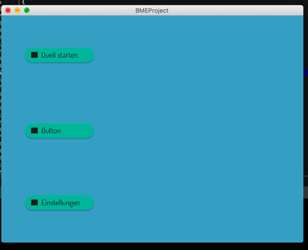
\includegraphics[width=5cm]{../img/screenshot_titlescreen.PNG} }}
\qquad
 \subfloat[Screenshot: Titlescreen 2]{{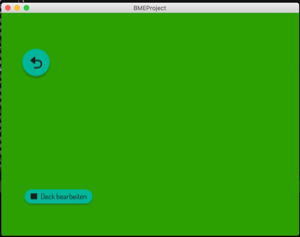
\includegraphics[width=5cm]{../img/screenshot_titlescreen_2.PNG} }}
\caption{Screenshots Titlescreen}%
 \label{fig:Screenshots Titlescreen}%
\end{figure}

In der render() Methode wird festgelegt, welcher Screen nach einem Klick auf den imageButtonBack angezeigt wird. In diesem Fall, soll das Startbildschirm erneut angezeigt werden. Nachdem mit einer If-Anweisung überprüft wird, ob der zurück Button geklickt wurde, wird das Startbildschirm angezeigt.  

Schließlich wurde durch diese Implementierung ermöglicht, die Spielumgebungen durch Klicks auf die Buttons anzusteuern und zwischen den Screens zu wechseln. 

\subsubsection{Imagebuttons für BattleScreen}
Anfangs wurden die Screens mit einer Hintergrundfarbe festgelegt. 
Allerdings war das nur vorübergehend. In diesem Semester erstellte Robert Sabo alles, was für den BattleScreen benötigt wurden.
Alle Bilder, die hierfür auf diesem Screen benötigen werden, wurden zunächst einmal in den Assets- beziehungsweise Visuals-Ordner eingefügt. Das Spielfeld sah anfangs an den Seiten leer aus. Das liegt daran, das alle Buttons hinzugefügt und richtig positioniert werden mussten. Das Endergebnis ist in Abbildung \ref{fig:Screenshot: BattleScreen mit ImageButtons} zu sehen.
\begin{figure}
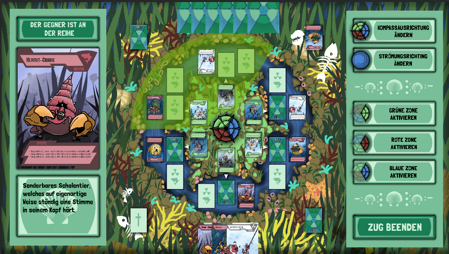
\includegraphics[width=0.5\textwidth]{../img/screenshot_battlescreen_buttons.PNG}
\caption{Screenshot: BattleScreen mit ImageButtons}
\label{fig:Screenshot: BattleScreen mit ImageButtons}
\end{figure}
Um testen zu können, ob der Klick auf den Button funktioniert, wurde zunächst einmal in der Console die Information „Zone successfully clicked“ wie folgt ausgegeben. \\
\begin{lstlisting}
450.0breite: 800.0
BATTLE SCREEN SHOWN
Zone successfully clicked
\end{lstlisting}

\subsubsection{Kartenauswahl}
Für die Auswahl einer bestimmten BattleCard und die damit verbundene Aktivierung bzw. Aktionsauslösung mussten erst entsprechende Vorbereitungen getroffen werden.
Zum einen benötigte die Klasse an sich einen InputListener des Typs “touchDown”, welcher für die Auswahl der Karte durch Anklicken benötigt wird. Das Hinzufügen des InputListeners stellte die Klasse Actor, von der die BattleCard erbt, über die Methode addListener bereit. Ihr musste nur die Klasse InputListener übergeben werden, bei der man direkt interne Anpassungen durchführen konnte. So wurde die von ihr beinhaltende Methode touchDown für unser Vorhaben genutzt, indem sie die von dem Klick betroffene Karte als “zuletzt angeklickte Karte” sicherte. Für eine flexiblere Verwendung der dadurch aktivierten Karte, wurde sie im BattleController als solche gesetzt und war damit dank Getter-Methoden auch von den restlichen Klassen abrufbar.

\subsubsection{Karte aus der Hand spielen}
Bei jedem Kartenspiel ist es wichtig, die Karte, welche aus der Hand gespielt wird, abzulegen. Um diese Funktionalität an der richtigen Stelle einbauen zu können, wurde zunächst einmal der Code analysiert. Mit Hilfe der Ausgabe auf der Consolen-Ausgabe, konnte ermittelt werden, welche Klassen und Methoden hierfür benötigt wurden. 

Die giveLastClickedBattledCard() Methode in der BattleControler Klasse gibt die lastClickedBattleCard, mit dem Rückgabetyp BattleCard, zurück. Mit Hilfe dessen, wurde zu aller erst ermittelt, ob die selecteCard null ist. Denn nur wenn eine Karte erst ausgewählt wird, kann diese auch wieder abgelegt werden. Nach einer weiteren if-Anweisung konnte mit Hilfe der Methoden addCard() und resetLastClicketBattleCard() die Funktionalität, die Karte aus der Hand zu legen, implementiert werden. Die folgenden Zeilen ermöglichen diesen Spielzug. 

\begin{lstlisting}
@Override public boolean touchDown(InputEvent event, float x, float y, int pointer, int button)
{
    BattleController battleController = FIELDABLE.giveBattleController();
    BattleCard  selectedCard     = battleController.giveLastClickedBattleCard();

    if (selectedCard != null) {
        addCard(selectedCard);
        battleController.resetLastClickedBattleCard();
    }
    return true;
}
\end{lstlisting}

Damit wurde somit dem Anwender die Option gegeben, seine Karte auf dem Spielfeld abzulegen. 

\subsubsection{TitleScreen ausbauen: zum BattleScreen navigieren}
Sobald das Projekt gestartet wurde, wurde uns der BattleScreen angezeigt. Daher musste der TitelScreen ausgebaut werden. Am Anfang des Semesters wurde diese Funktionalität zwar bereits programmiert, allerdings gab es während dem Semester Code-Änderungen. Das Resultat dieser Änderungen ergab, dass trotz eines Klicks auf den Button, der Anwender weiterhin den Titelbildschirm sah und somit nicht navigiert wurde. 

Dabei wurde festgestellt, dass der Verweis auf den BattleScreen nicht sofort funktionierte, weshalb der vorhandene Code analysiert wurde. Der TitelScreen erbt von AbstractScreen. Dieser enthält die Methode createController mit dem Parameter SpriteBatch spriteBatch. Allerdings muss diese Methode in der TitelScreen Klasse erweitert werden. Daher musste der Konstruktor der TitelController Klasse mit einem zweiten Parameter, dem TitelScreen titelScreen, ergänzt werden. Des Weiteren wurde im TitelScreen der return Wert von der creatController Methode angepasst. Schließlich funktionierte wieder der Verweis auf den BattleScreen. 

\subsubsection{Deckeditor}
Um dem Spieler die Möglichkeit zu verschaffen ein eigenes, individuelles Spielkartendeck zu erstellen, war anfangs ein Deckeditor geplant, der vom Titelscreen aus aufgerufen werden sollte. Die Klassen Deck, DeckScreen und DeckController wurden hierfür implementiert. Sie waren anfangs auch für interne Tests hilfreich, da sie alle Spielkarten hielten und dadurch der Zugriff auf Daten wie Kartenname oder Typ möglich war. Da die Priorität am Ende jedoch auf einer funktionierenden, visuell ansprechenden Spielfunktion lag, wurde der Deckeditor, und damit auch die Ausarbeitung der Deck-Klassen, auf Eis gelegt.

\subsubsection{Karten ziehen (Debug)}
Zur Visualisierung der Kartenziehung wurde vorerst vom Kartenstapel jeweils eine Karte auf das HandField verschoben.
Dafür musste die drawTopCard-Methode der Player-Klasse innerhalb des BattleControllers aufgerufen werden.
Dieser Aufruf musste nur noch mittels eines Impuls ausgelöst werden, für diesen Fall bot sich die von LibGDX bereitgestellte Tastendruckabfrage an:
\begin{lstlisting}
if (Gdx.input.isKeyJustPressed(Input.Keys.SPACE)) {
	activePlayer.drawTopCard();
}
\end{lstlisting}
Vorerst wurde diese Aktion mittels der Leertaste ausgeführt, wobei der Auslöser im Laufenden noch ausgearbeitet wurde.

\subsubsection{Visuelles Feedback innerhalb Eintrittsfelder}
Um dem Nutzer das Spielprinzip während seines Spielzuges zu erleichtern, bot sich eine visuelle Rückmeldung für die zum Ablegen von BattleCards ansteuerbaren Felder an. Um die Aufmerksamkeit des Nutzers also auf die möglichen Ablageorte zu lenken, wurde als Form der Kennzeichnung ein Asset in Form eines gelben Rahmens mit glühendem Effekt angefertigt. Dieses wird schließlich um das Feld oder die Felder pulsartig aufleuchten.
Der erste Schritt in der Implementierung dieser Funktion lag im Hinzufügen des Assets in alle Ablagefelder (EntryFields), wobei seine Transparenz auf Null gesetzt wurde. Optisch änderte sich am Spielfeld also noch nichts.
Bei diesem Schritt kam es jedoch zum Problem, dass sich das Verhalten des Ablagefeldes funktional veränderte, so wurde ein Mausklick auf dieses nicht mehr erkannt. Ein Kartenablegen auf dieses Feld war damit unmöglich.
Der Fehler lag hierbei in der Positionierung des Assets, das fälschlicherweise über den Feld-Actor gelegt wurde, der den Mausklick erhält. Dafür musste man die Assets auf eine niedrigere Ebene als die des Actors legen. Für diese Positionierung setzte man die Z-Position der Assets neu:
\begin{lstlisting}
int zCor = getZIndex() - 1;
glowBorder.setZIndex(zCor);
\end{lstlisting}

Der zweite Schritt wird durch den Mausklick auf die BattleCard angestoßen. Hier wird vorerst durch alle sechs Sektoren durchiteriert:

\begin{lstlisting}
public void activateSectorOfPlayer(Party party){
  for (Sector s : BATTLEFIELD.giveSectors()) {
     if (s.giveCommander().PARTY == party) {
        s.giveEntryField().showBorder();
     } else {
        s.giveEntryField().hideBorder();
     }
  }
}
\end{lstlisting}

Liegt dabei ein Sektor im Besitz des aktiven Spielers, so startet die vorgesehene Animation auf dem im Sektor enthaltenen Ablagefeld.
Für Animationen stellt LibGDX eigene Aktionen bereit. Für den gewünschten, pulsierenden Effekt wurde die “RepeatAction” gewählt, der man eine Ausblende- und Einblendefunktion übergeben muss:

\begin{lstlisting}
repeatAction.setAction(Actions.sequence(Actions.fadeOut(duration);
Actions.fadeIn(duration)));
\end{lstlisting}

Bei jedem Aufruf dieser Aktion werden diese beiden Funktionen einer Art Aktionsschleife hinzugefügt. Je länger diese Schleife wuchs, desto geringer wurde der prozentuale Anteil der Animationsdauer (Duration), daher verschnellerte sich bei jedem Klick die Rahmenanimation des Ein- und Ausblendens. Aus diesem Grund musste diese Aktionsschleife vor jedem Aufruf zuerst geleert werden:

\begin{lstlisting}
glowBorder.getActions().clear();
\end{lstlisting}

Diese Methode wird auch für das Beenden der Animation verwendet. Dieser Fall tritt immer dann ein wenn der Spieler aktuell keine BattleCard aktiviert hat, also wenn er entweder eine Karte abgelegt oder sie durch Klicken auf das Spielfeld unselektiert hat.
Das Beenden der Animation lässt den Rahmen jedoch nicht verschwinden, sondern fügt ihn in seiner aktuellen Transparenz, die zwischen Eins (fadeIn) und Null (fadeOut) variiert, der Stage hinzu. Für das endgültige Beenden der visuellen Rückmeldung muss die Transparenz der Assets wieder auf Null gesetzt werden:

\begin{lstlisting}
glowBorder.setColor(1,1,1,0);
\end{lstlisting}

\subsubsection{Klickanimation der Buttons}
Für die visuelle Bestätigung der Durchführung eines Klicks wurden die Spielefeldbuttons um ein Asset erweitert. Der Aufruf des ImageButton-Konstruktors mit zwei Parametern, imageUp und imageDown, ermöglicht es die Buttongrafiken während eines Mausklicks, als auch nach dieser Aktion, zu setzen. Das neu hinzugefügte Asset beinhaltet die Buttongrafik in einer schwächeren Belichtung:

\begin{lstlisting}
final Texture     BUTTON_RED_DOWN = new Texture("core/assets/visuals/buttons/3_rotbuttonSmall_down.png");
final ImageButton RED_BUTTON = new ImageButton(new TextureRegionDrawable(new TextureRegion(BUTTON_RED)), new TextureRegionDrawable(new TextureRegion(BUTTON_RED_DOWN)));
\end{lstlisting}

\subsubsection{Deselektion der BattleCard}
Selektiert der Player eine Handkarte und entscheidet sich daraufhin um, weil er lieber eine oder mehrere andere Aktionen durchführen möchte, wird der Buffer der letzten geklickten Karte geleert und ihre Aktivierung damit aufgehoben. Generell geschieht dies bei jedem Mausklick außerhalb einer BattleCard.
Benötigt wird hier also eine Abfrage, ob sich auf geklickter Position ein Actor befindet, der wiederum von einer BattleCard gehalten wird.
Mit der hit-Methode der Stage-Klasse können wir dies leicht überprüfen. Diese benötigt lediglich die Koordinaten des Mausklicks, um einen dort positionierten Actor auszugeben. Dieser wird anschließend auf seine Zugehörigkeit geprüft, die nicht der BattleCard angehören darf:

\begin{lstlisting}
if (Gdx.input.justTouched()) {
	Stage stage = giveStage();
	Vector2 vector = new Vector2(Gdx.input.getX(), Gdx.input.getY());
	stage.screenToStageCoordinates(vector);
	Actor clickedActor = stage.hit(vector.x, vector.y, true);
	if (clickedActor != null){
		if(!(clickedActor instanceof BattleCard)) {
			resetLastClickedBattleCard();
		}
	}
}
\end{lstlisting}